\documentclass[a4paper,12pt]{article} 
\usepackage[T2A]{fontenc}			
\usepackage[utf8]{inputenc}			
\usepackage[english,russian]{babel}	
\usepackage{amsmath,amsfonts,amssymb,amsthm,mathrsfs,mathtools} 
\usepackage{cancel}
\usepackage{multirow}
\usepackage[colorlinks, linkcolor = blue]{hyperref}
\usepackage{upgreek}\usepackage[left=2cm,right=2cm,top=2cm,bottom=3cm,bindingoffset=0cm]{geometry}
\usepackage{tikz}
\usepackage{graphicx}
\usepackage{subfig}
\usepackage{titletoc}
\usepackage{pgfplots}
\usepackage{xcolor}
\usepackage{wrapfig}
\author{Дорогинин Д.В.\\
Группа Б02-825}
\title{4.7.2. Эффект Поккельса}
\date{}

%\begin{wrapfigure}{r}{0.5\textwidth}
%\begin{center}
%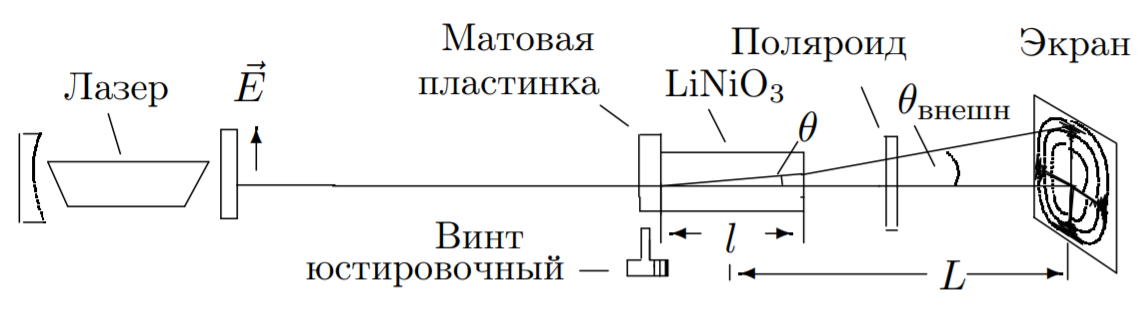
\includegraphics[width = 0.4\textwidth]{1.png}
%\end{center}
%\caption{}
%\end{wrapfigure}

\begin{document}
\maketitle
\textbf{Цель работы}: исследовать интерференцию рассеянного света, прошедшего кристалл; наблюдать изменение характера поляризации света при наложении на кристалл электрического поля.


\textbf{В работе используются}: гелий-неоновый лазер, поляризатор, кристалл ниобата лития, матовая пластина, экран, источник высоковольтного переменного и постоянного напряжения, фотодиод, осцилограф, линейка.
\section*{Теория}
Эффект Поккельса -- изменение показателя преломления света в кристалле под действием электрического поля.\\
Рассмотрим кристалл ниобата лития $\text{LiNbO}_3$ с цетрольноосевой симметрией вдоль оси $Z$. Для световой волны с $\mathbf{E}$ перпендикулярно $Z$ показатель преломления будет $n_o$, а для волны с $\mathbf{E}$ вдоль $Z$ -- $n_e$. В случае, когда луч света идёт под углом $\theta$ к оси, есть два значение показателя преломления $n_1$ и $n_2$: $n_1 = n_o$ для волны с $\mathbf{E}$ перпендикулярным плоскости $(\mathbf{k},\mathbf{Z})$ (обыкновенная волна) и $n_2$ для волны с $\mathbf{E}$ в этой плоскости (необыкновенная волна). В последнем случае
\begin{equation}
\dfrac{1}{n_2^2}=\dfrac{\cos^2 \theta}{n_0^2}+\dfrac{\sin^2 \theta}{n_e^2}.
\end{equation}

\begin{wrapfigure}{r}{0.4\textwidth}
\begin{center}
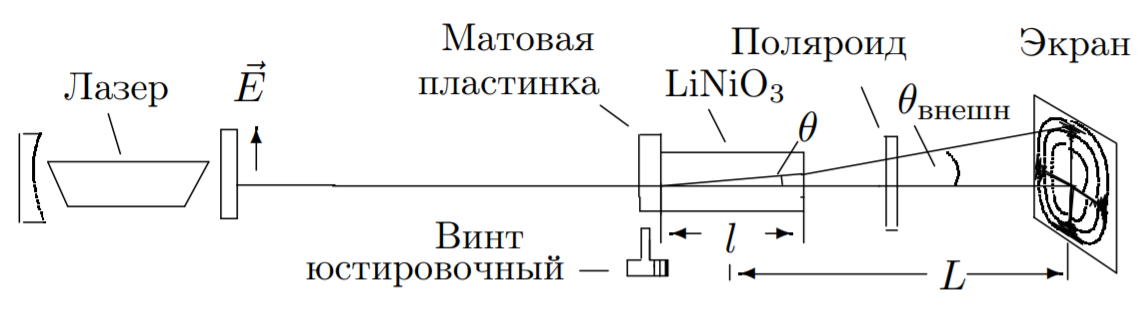
\includegraphics[width = 0.4\textwidth]{1.png}
\end{center}
\vspace{-40ptx}
\caption{Схема для наблюдения интерфереционной картины.}
\end{wrapfigure}
%\begin{figure}[h!]
%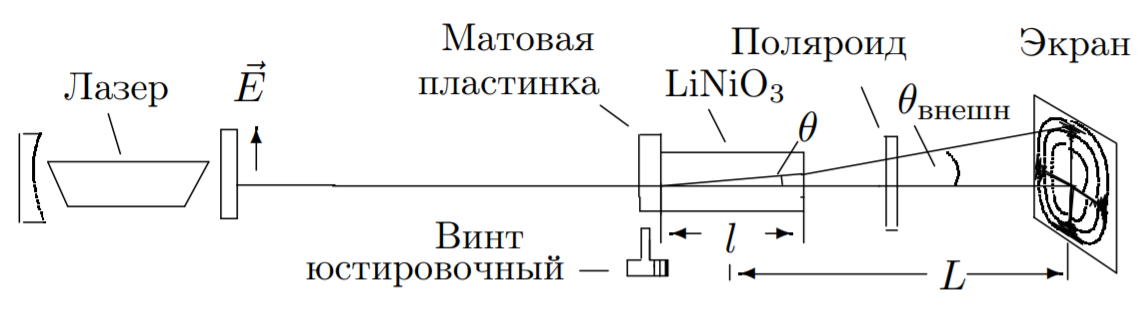
\includegraphics[scale=0.5]{1.png}
%\centering
%\caption{Схема для наблюдения интерфереционной картины}
%\end{figure}
Если перед кристаллом, помещённым между поляроидами, расположить линзу или матовую пластинку, то на экране за поляроидом мы увидим тёмные концентрические окружности -- рещультат интерфернции обыкновенной и необыкновенной волн. При повороте выходного поляроида на $90^\circ$ картина меняется с позитива на негатив (на месте светлых пятен тёмные и наоборот). В случаи, когда разрешённое направление анализатора перпендикулярно поляризации лазерного излучения, радиус тёмного кольца с номером $m$ равен
\begin{equation}
r_m^2 = \dfrac{\lambda}{l} \dfrac{(n_oL)^2}{n_0 - n_e}m,
\end{equation}
где $L$ -- расстояние от центра кристалла до экрана, $l$ -- длина кристалла.\\
Теперь поместим кристалл в постоянное электрическое поле $E_{\text{эл}}$, направленное вдоль оси $X$, перпендикулярной $Z$. Показатель преломления для луча, распространяющего вдоль $Z$, всегда $n_o$. В плоскости $(X,Y)$ возникают два главных направления под углами $45^\circ$ к $X$ и $Y$ с показателями преломления $n_0 - \Delta n$ и $n_o + \Delta n$ (быстрая и медленная ось), причём $\Delta n = A E_{\text{эл}}$. Для поляризованного вертикально света и анализатора, пропускающего горизонтальную поляризацию, на выходе интенсивность на выходе будет иметь вид
\begin{equation}
I_{\text{вых}} = I_0 \sin^2 \left(\dfrac{\pi}{2} \dfrac{U}{U_{\lambda/2}} \right),
\end{equation}
где $U_{\lambda/2} = \frac{\lambda}{4A}\frac{d}{l}$ -- \textit{полуволновое напряжение}, $d$ -- поперечный размер кристалла.  При напряжении $U = E_{\text{эл}}d$ равном полуволновому сдвиг фаз между двумя волнами равен $\pi$, а интенсивность света на выходе максимальна. 


\begin{wrapfigure}{r}{0.45\textwidth}
\begin{center}
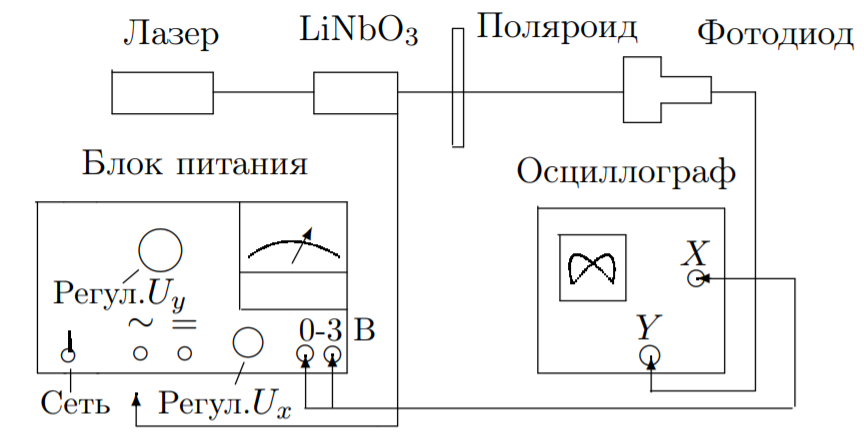
\includegraphics[width = 0.45\textwidth]{2.png}
\end{center}
\vspace{-40ptx}
\caption{Схема установки.}
\end{wrapfigure}
На Рис. 2 представлена схема всей установки (оптическая часть изорбажена на Рис. 1). Свет лазера, проходя через сквозь пластину, рассеивается и падает на двоякопреломляющий кристалл. На экране за поляроидом видна интерференционная картина. Убрав рассеивающую пластину и подавая на кристалл постоянное напряжение, можно величиной напряжения влиять на поляризацию луча, вышедшего из кристалла. Заменив экран фотодиодом и подав на кристалл переменное напряжение, можно исследовать поляризацию с помощью осциллографа.
\newpage
\section*{Ход работы}
В схеме согласно Рис. 1 получим интерфереционную картину. Радиусы $r(m)$ тёмных колец при расстоянии $L = 60 \text{ см}$ приведены в Таблице 1. На Рис. 3(б) изображён график $r^2 = f(m)$.
%\begin{wrapfigure}{r}{0.5\textwidth}
%\begin{center}
%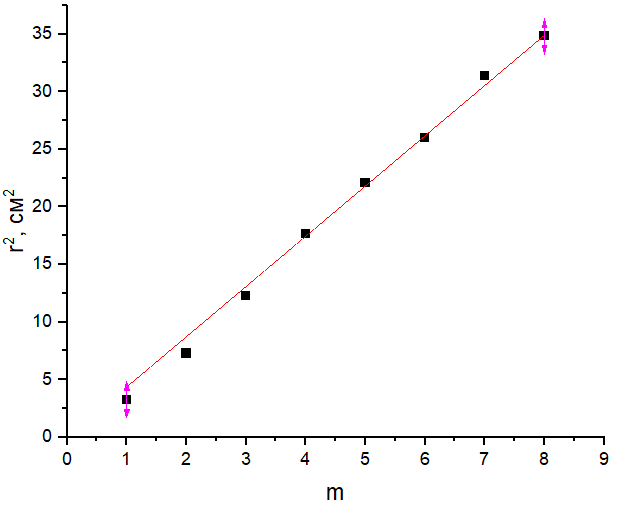
\includegraphics[width = 0.45\textwidth]{3.png}
%\end{center}
%\vspace{-40pt}
%\caption{Зависимость $r^2 = f(m)$.}
%\end{wrapfigure}
\begin{table}[h]
\begin{tabular}{|c|c|c|c|c|c|c|c|c|}
\hline
$m$     & 1   & 2   & 3   & 4   & 5   & 6   & 7   & 8   \\ \hline
$r_m$, см & 1.8 & 2.7 & 3.5 & 4.2 & 4.7 & 5.1 & 5.6 & 5.9 \\ \hline
\end{tabular}
\centering
\caption{Радиусы тёмных колец.}
\end{table}\\
Из МНК угловой коэффициент получаем $k = 4.36 \pm 0.04 \text{ см}^2$. Отсюда для значений $n_0 = 2.29$, $\lambda = 0.63 \text{ мкм}$, $l = 26 \text{ мм}$ получаем из формулы (2)
$$
n_0 - n_e = 0.105\pm 0.010. 
$$  
На установке по Рис. 2 определим полуволновое напряжение по разности напряжений при максимуме и минимуме у фигуры Лиссажу: $U_{\lambda/2} = 450 \pm 15 \text{ В}$. 
Подавая на кристалл $U_{\lambda/4} = \frac{1}{2}U_{\lambda/2}$, убеждаемся, что поляризация круговая.\\
Вид фигуры Лиссажу, наблюдаемой на осциллографе, представлен на Рис. 3(а). Первый минимум соответсвует $U_{\lambda/2}$, максимум -- $U_{\lambda}$, второй минимум -- $U_{3\lambda/2}$. При изменение полярности поляроида картина отображается симметрично оси $OX$.
%\begin{wrapfigure}{r}{0.5\textwidth}
%\begin{tikzpicture}
%\begin{axis}[
%    axis lines=middle,
%    xticklabels={,,},
%    yticklabels={,,},
%    xmin = -4,
%    xmax = 4,
%    ymin = -2,
%    ymax = 2,
%    axis line style={draw=none},
%    tick style={draw=none}
%]
%\draw (axis cs:0,0) to [out=-80,in=180] (axis cs:0.5,-0.7);
%\draw (axis cs:0.5,-0.7) to [out=0,in=180] (axis cs:1.9,0.7);
%\draw (axis cs:1.9,0.7) to [out=0,in=120] (axis cs:2.6,-0.7);
%\draw (axis cs:0,0) to [out=-70,in=180] (axis cs:0.6,-0.7);
%\draw (axis cs:0.6, -0.7) to [out=0,in=180] (axis cs:1.8,0.7);
%\draw (axis cs:1.8,0.7) to [out=0,in=115] (axis cs:2.6,-0.7);
%
%\draw (axis cs:0,0) to [out=-100,in=0] (axis cs:-0.5,-0.7);
%\draw (axis cs:-0.5,-0.7) to [out=180,in=0] (axis cs:-1.9,0.7);
%\draw (axis cs:-1.9,0.7) to [out=180,in=50] (axis cs:-2.6,-0.7);
%\draw (axis cs:0,0) to [out=-110,in=0] (axis cs:-0.6,-0.7);
%\draw (axis cs:-0.6, -0.7) to [out=180,in=0] (axis cs:-1.8,0.7);
%\draw (axis cs:-1.8,0.7) to [out=180,in=65] (axis cs:-2.6,-0.7);
%\end{axis}
%%\end{tikzpicture}
%\centering
%\caption{Вид фигуры Лиссажу.}
%\end{wrapfigure}
\begin{figure}[h]
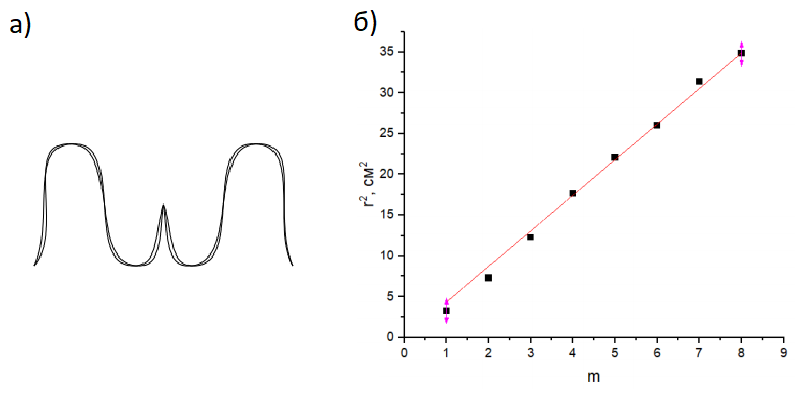
\includegraphics[scale=0.9]{4.png}
\centering
\caption{(а) Вид фигуры Лиссажу. (б) Зависимость $r^2 = f(m)$.}
\end{figure}
\end{document}